%--- document format ---%
\documentclass[             % for every option see KOMA-Script Guide
    final,                  % final / draft (for fast compilation without images)
    ngerman,                % set main language globally, see options of babel package
    paper=A4,               % paper size
    paper=portrait,         % paper orientation: portrait / landscape (use landscape with option oneside)
    twoside,                % oneside / twoside (for books)
    open=right,             % begin chapters on specified side if twoside is enabled: any, right, left
    onecolumn,              % single column text, twocolumn
    fontsize=11pt,          % font size to use
    BCOR=7.5mm,               % binding correction
    DIV=10,                 % size of text area (fontsize=11pt -> DIV=10, see KOMA-Script Guide)
    titlepage=true,         % no \newpage after \maketitle
    toc=bib,                % add bibliography to table of contents
    toc=idx,                % add index to table of contents
    toc=listof,             % add list of figures / tables / listings to table of contents
    chapterentrydots=false, % dots in table of contents for chapters
    numbers=noendperiod,    % no period at the end of arabic part numbering
    captions=signature,     % format everything with a signature
    captions=figuresignature,   % heading on top of figure: figureheading, signature on bottom: figuresignature
    captions=tableheading,  % heading on top of table: tableheading, signature on bottom: tablesignature
    captions=nooneline,     % multicolumn caption: nooneline, single column: oneline
    bibliography=openstyle, % oldstyle (compact form), openstyle (better reading)
    automark                % chapter and section names in header
]{scrbook}                  % base document is book

%--- monochrome setting for print ---%
\newcommand{\true}{1}
\newcommand{\false}{0}
\newcommand{\isdigital}{\true} % \true (digital pdf) or \false (monochrome print version)

%--- packages ---%
\if\isdigital\false
    \usepackage[monochrome]{color}
\fi

\usepackage{scrhack}            % improved compatibility for KOMA-Script with float and babel
\usepackage[utf8]{inputenc}     % encoding of the input files
\usepackage[T1]{fontenc}        % internal charset
\usepackage[                    % set document language
    main=ngerman,               % main language is german
    english                     % also support for english
]{babel}                        % language of document, main is ngerman and in addition there may be some english words
\usepackage{lmodern}            % nicer set of fonts
\usepackage[normalem]{ulem}     % different styles for underline text
\usepackage{amsfonts}
\usepackage{amssymb}
\usepackage{amsmath}
\usepackage{amsthm}
\usepackage{dsfont}             % double stroke mathematical symbols like N, Z, Q, R, C
\usepackage{mathtools}
\usepackage{geometry}
\usepackage{setspace}           % for line spacing: singlespacing, onehalfspacing
\usepackage{float}              % floating environments and options
\usepackage{caption}            % formatting captions
\usepackage{longtable}          % for multipage tables
\usepackage{svg}                % for including svg files
\usepackage{graphicx}           % for including graphics
% \usepackage[
%     usenames,
%     dvipsnames,
%     table,
%     xcdraw
% ]{xcolor}             % define and use colors
\usepackage{scrlayer-scrpage}   % page header and footer
\usepackage[
    marginal,
    stable
]{footmisc} % change footnote style
\usepackage[
    backend=biber,
    style=alphabetic,
    natbib=true, % comma separated
    backref=page % page references in bibliography
]{biblatex} % bibliography environment
\usepackage[
    hyperfootnotes=true,
    breaklinks=true,
    linktoc=all,
    colorlinks=true,
    unicode=true
]{hyperref} % links
\usepackage{cleveref} % for label and ref commands
\usepackage{soulutf8} % backgroundcolor, textcolor
\usepackage[newfloat]{minted} % minted for source code presentation
\usepackage{csquotes} % enqoute text properly
\usepackage{array} % format tables
\usepackage{diagbox} % diagonal split box in table
\usepackage{ragged2e} % Centering, RaggedRight, etc
\usepackage{tikz} % drawing package for shapes, etc
\usepackage{enumitem} % includes enumerate package
\usepackage{pdfpages} % for including pdf pages into the document
\usepackage{afterpage} % command execution after next page break
\usepackage{acronym} % for acronyms list and ref in text
\usepackage{makeidx} % for indexing words
\usepackage{blindtext} % FOR TESTING PURPOSES ONLY

%--- constants ---%

%--- settings ---%
\setcounter{tocdepth}{\paragraphtocdepth}       % part to paragraph in table of contents
\setcounter{secnumdepth}{\paragraphtocdepth}    % numbering from part down to paragraph
\setlength\parindent{0pt}                       % no indentation at sections
\captionsetup{format=plain,indention=1.5em,font=small,labelfont=bf} % setup caption look
% define list icons for itemize
\renewcommand{\labelitemi}{\raisebox{0.2ex}{$\bullet$}}
\renewcommand{\labelitemii}{\raisebox{0.2ex}{$\circ$}}
\renewcommand{\labelitemiii}{\raisebox{0.5ex}{\tiny$\bullet$}}
\renewcommand{\labelitemiv}{\raisebox{0.5ex}{\tiny$\circ$}}
% some colors for links and code
\definecolor{darkred}{rgb}{0.6, 0, 0}
\definecolor{darkblue}{rgb}{0, 0, 0.6}
\definecolor{lightgrey}{gray}{0.875}
\pagestyle{scrheadings}                         % standard scr headings on page
\hypersetup{
    allcolors=darkred, % implicit: linkcolor=darkred,citecolor=darkred
    urlcolor=darkblue
} % setup of link colors
\setminted{
    frame=lines,
    framesep=2mm,
    baselinestretch=1.2,
    fontsize=\footnotesize,
    linenos,
    breaklines=true
} % setup minted environment
\useunder{\uline}{\ul}{} % for ulem

% biblatex break links on page width and add resources
\setcounter{biburlnumpenalty}{100}
\setcounter{biburlucpenalty}{100}
\setcounter{biburllcpenalty}{100}
\bibliography{quellen.bib}

% setup caption height
\setlength{\abovecaptionskip}{10pt}
\setlength{\belowcaptionskip}{15pt}

% setup floating environment [h] height
\setlength{\intextsep}{15pt}

% setup index
\makeindex
\AtBeginDocument{\renewcommand{\indexname}{Stichwortverzeichnis}}

%--- workarounds ---%
% footmisc and hyperref: multiple
\let\oldFootnote\footnote
\newcommand\nextToken\relax
\renewcommand\footnote[1]{%
    \oldFootnote{#1}\futurelet\nextToken\isFootnote}
\newcommand\isFootnote{%
    \ifx\footnote\nextToken\textsuperscript{,}\fi}

%--- own commands ---%
% command
% new frontmatter, mainmatter, backmatter commands

% make full reference with number and text
% dependencies: hyperref
\newcommand*{\fullref}[1]{\hyperref[{#1}]{\ref*{#1} \nameref*{#1}}}
\newcommand*{\figfullref}[1]{\hyperref[{#1}]{Abbildung \ref*{#1}: \nameref*{#1}}}
\newcommand*{\tablefullref}[1]{\hyperref[{#1}]{Tabelle \ref*{#1}: \nameref*{#1}}}
\newcommand*{\codefullref}[1]{\hyperref[{#1}]{Quellcode \ref*{#1}: \nameref*{#1}}}

% command for marking inline code
% dependencies: soulutf8
\newcommand{\inlinecodetext}[2]{
  \begingroup
  \sethlcolor{#1}
  \hl{#2}
  \endgroup
}
% \newcommand{\inlinecodecolor}{\if\isdigital\true lightgrey\else white\fi}
\if\isdigital\true
    \newcommand{\inlinecode}[1]{\inlinecodetext{lightgrey}{\texttt{ #1 }}}
\else
    \newcommand{\inlinecode}[1]{\texttt{ #1 }}
\fi

% define code environment
\newcounter{codectr}\setcounter{codectr}{0}
\newenvironment{code}{
    \captionsetup{type=listing,font=small,labelfont=bf,skip=0pt}
    \refstepcounter{codectr}
}{}
\newfloat{code}{H}{code}[chapter]
\floatname{code}{Quellcode}

% define column width
% dependencies: array
\newcolumntype{L}[1]{>{\raggedright\let\newline\\\arraybackslash\hspace{0pt}}m{#1}}
\newcolumntype{C}[1]{>{\centering\let\newline\\\arraybackslash\hspace{0pt}}m{#1}}
\newcolumntype{R}[1]{>{\raggedleft\let\newline\\\arraybackslash\hspace{0pt}}m{#1}}

% encircle text with command circled
% dependencies: tikz
\newcommand*\circled[1]{\tikz[baseline=(char.base)]{
            \node[shape=circle,draw,inner sep=1.5pt] (char) {#1};}}
            
% readable indexing with \Index{...}, no duplicate words
\newcommand{\Index}[1]{#1\index{#1}}

%--- document information ---%
\subject{Thema}
\title{Titel}
\subtitle{Untertitel}
\author{Autor}
\date{\today}

%--- actual document ---%
\begin{document}

% title page and table of contents
\singlespacing

\maketitle
\tableofcontents

\addchap{Abkürzungsverzeichnis}
\begin{acronym}[LargestWord]
    \acro{ABC}{Alphabet}
\end{acronym}

\onehalfspacing
\addchap{Abstract}
\blindtext % FOR TESTING PURPOSES ONLY

% text part
\onehalfspacing

\chapter{KapABC}
\blindtext % FOR TESTING PURPOSES ONLY
\footnote{siehe \cite{ford}}
\section{AbsABC}
\blindtext % FOR TESTING PURPOSES ONLY
\subsection{Unterabschnitt}
\blindtext
\footnote{\blindtext}\footnote{a}\footnote{b}
\enquote{gedruckten} Seitenzahlen sind Referenzen \circled{auf} die Definition
\inlinecode{PERFORM}
\footnote{\blindtext}

\begin{code}
\begin{minted}{abap}
REPORT Z_SELECT.

* Struktur aus Tabelle und Counter deklarieren *
DATA: ls_zpersonen TYPE ZPERSONEN,
      lv_nummer TYPE i VALUE 1.

* Datenbank abfragen und zwischenspeichern in Struktur *
SELECT * FROM ZPERSONEN INTO ls_zpersonen.
*   * Aufruf der Subroutine *
    PERFORM print_person USING ls_zpersonen lv_nummer.

*   * Counter um 1 inkrementieren *
    ADD 1 TO lv_nummer.
ENDSELECT.

* Routine für die Ausgabe *
FORM print_person
    USING f_zpersonen LIKE ZPERSONEN
          f_nummer LIKE i.
          
*   * Ausgabe der Daten auf der Konsole *
    WRITE:/ f_nummer, '. ',
            f_zpersonen-vorname, ' ',
            f_zpersonen-name, ': ',
            f_zpersonen-beruf.
ENDFORM.
\end{minted}
\caption{Unterprogramme aufrufen}
\label{code:perform}
\end{code}

\begin{figure}[H]
    \centering
    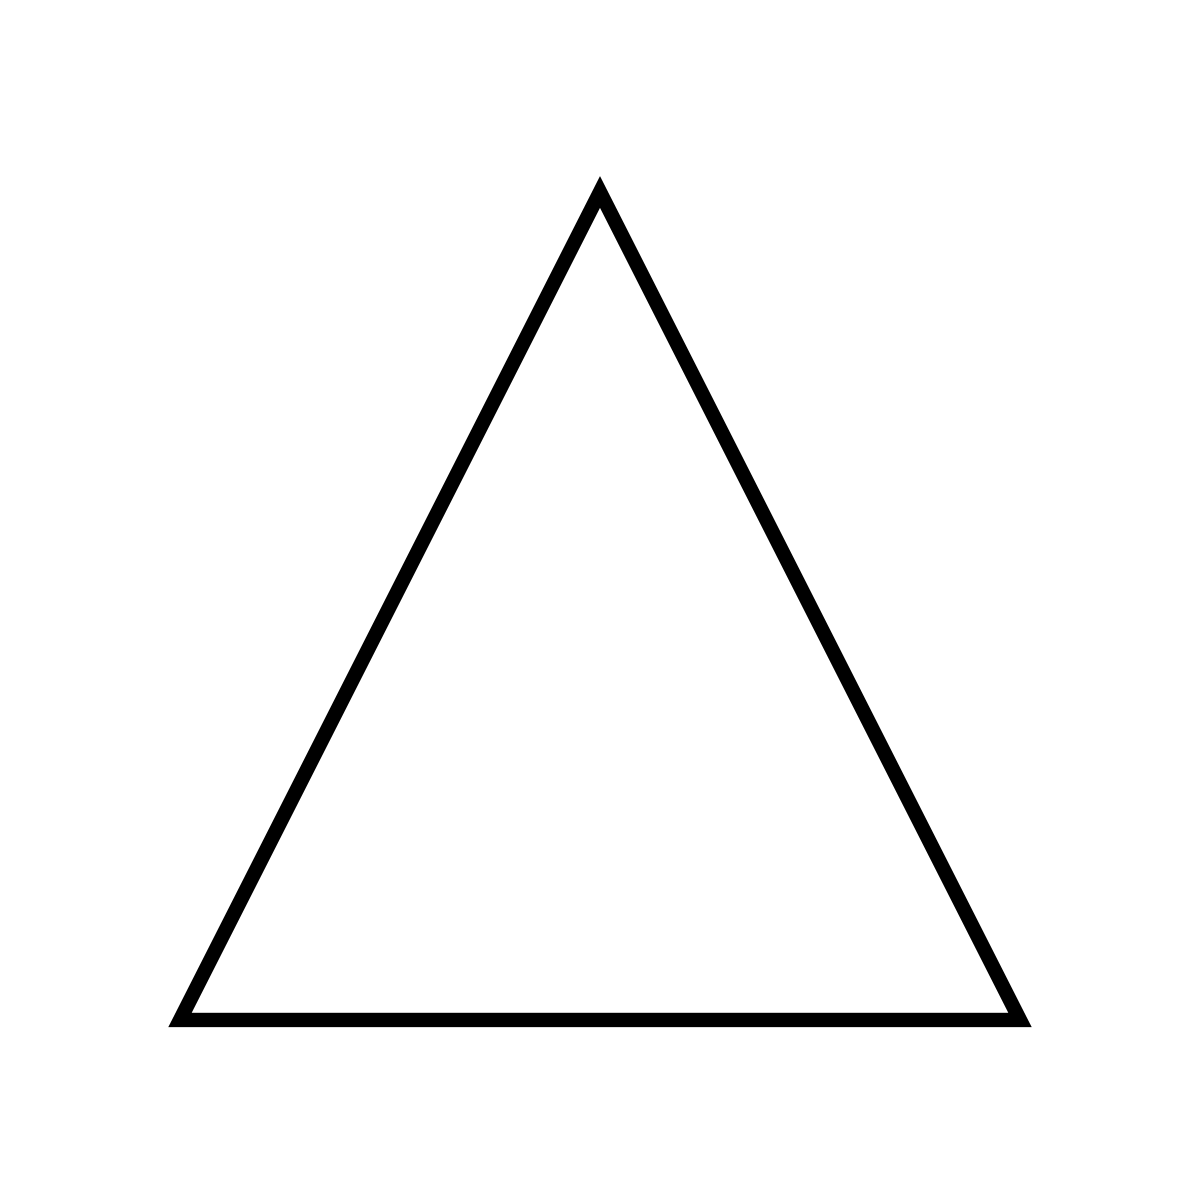
\includegraphics[width=0.5\textwidth]{test.png}
    \caption{\blindtext}
    \label{fig:my_label}
\end{figure}
\subsubsection{Unterunterabschnitt}
\blindtext % FOR TESTING PURPOSES ONLY
\begin{itemize}
    \item \Index{blah}
    \begin{itemize}
        \item blah \acs{ABC}
        \begin{itemize}
            \item blah
            \begin{itemize}
                \item blah
            \end{itemize}
        \end{itemize}
    \end{itemize}
\end{itemize}
\blindtext \cite{gon}
\begin{table}[H]
    \centering
    \begin{tabular}{|l|l|l|}
        \hline
        \multicolumn{3}{|c|}{\texttt{ZPERSONEN}}\\\hline
        \texttt{name} & \texttt{vorname} & \texttt{beruf}\\\hline
        Anders & Malte & Backend-Entwickler\\
        Stein & Lara & Designerin\\
        Klein & Jan & Programmierer\\
        Schmidt & Merle & Softwaretesterin\\\hline
    \end{tabular}
    \captionsetup{type=table,font=small,labelfont=bf,skip=0pt} %%%%% problem not automatic
    \setlength{\abovecaptionskip}{10pt} %%%%% problem not automatic
    \setlength{\belowcaptionskip}{15pt} %%%%% problem not automatic
    \caption{Tabelle mit Beispieldaten}
    \label{table:personen}
\end{table}

\paragraph{Paragraf}
\blindtext % FOR TESTING PURPOSES ONLY

\boxed{\texttt{F}}

\begin{flushright}
$\blacksquare$\\
\end{flushright}

\begin{enumerate}
    \item Einführung (ca. 5 Seiten)
        \begin{enumerate}[label*=\arabic*.]
            \item Problemstellung
                \begin{enumerate}[label*=\arabic*.]
                    \item Kontext
                    \item Beschreibung
                \end{enumerate}
            \item Ziele und Fragen
            \item Abgrenzung
        \end{enumerate}
    \item Grundlagen (ca. 10 Seiten)
\end{enumerate}


\begin{tabular}{L{5.5cm} C{0.5cm} L{7.5cm}}
    Altenholz, 12.02.2019 & & \\
    \cline{1-1}\cline{3-3}
    \texttt{Ort, Datum} & & \texttt{Unterschrift Student}
\end{tabular}

\afterpage{
    \newgeometry{margin=0.25cm}
    
    \begin{figure}[H]
        \centering
        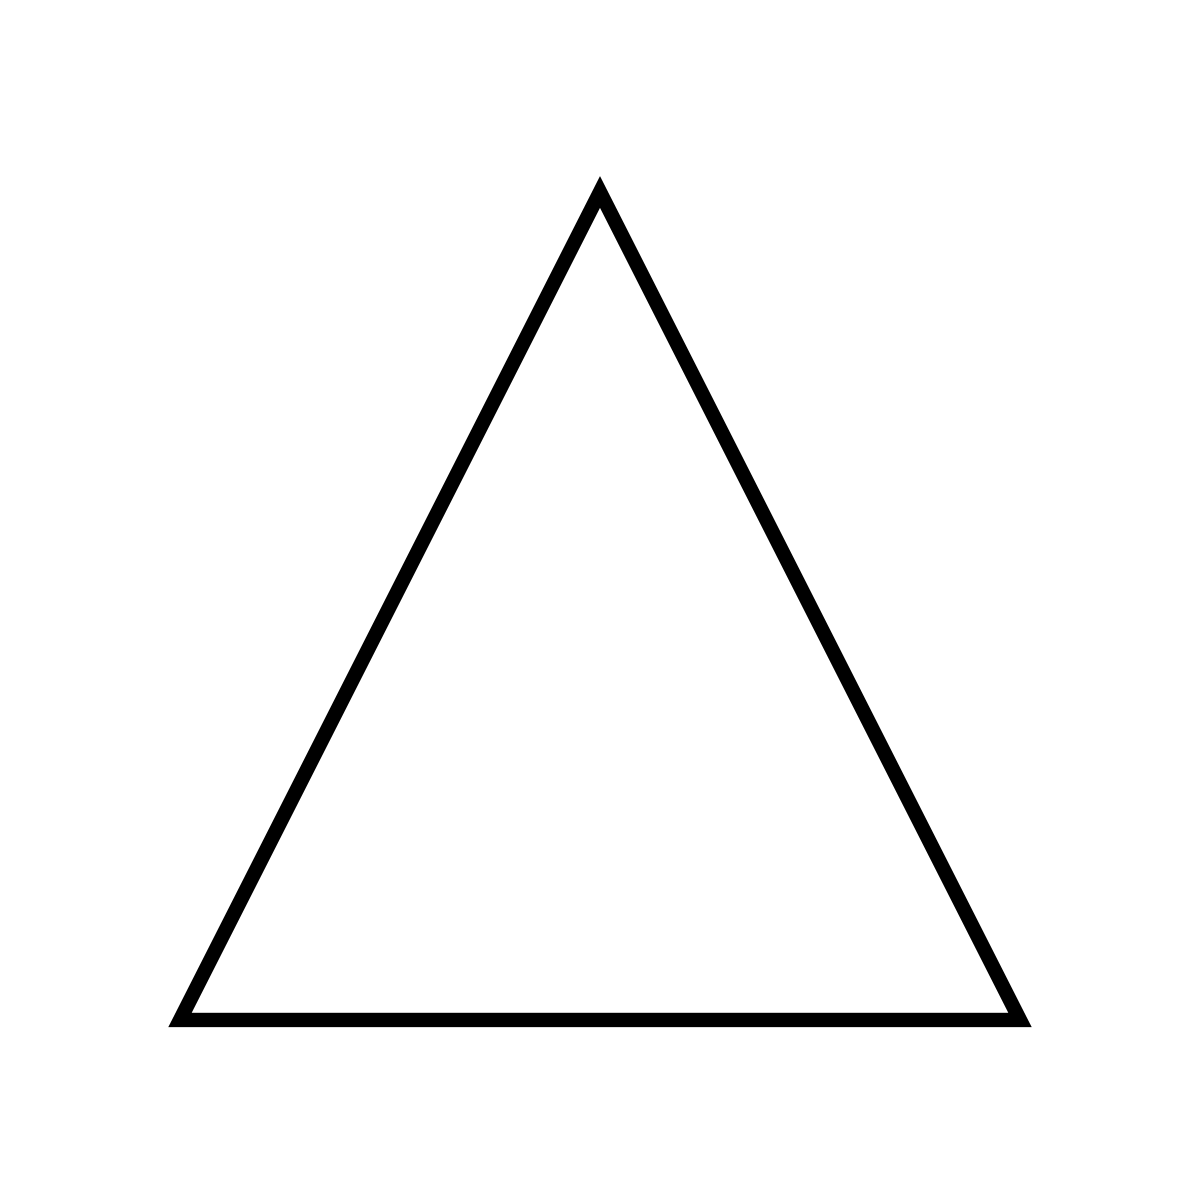
\includegraphics[angle=90,scale=0.5]{test.png}
        \caption{Zeitplan für die Thesis}
        \label{zeitplan}
    \end{figure}
    
    \clearpage
    \restoregeometry
}\restoregeometry\newpage

% /appendix /chapter{...}

% lists
\singlespacing

%Abkürzungsverzeichnis
\setindexpreamble{Alle \textbf{fett} gedruckten Seitenzahlen sind Referenzen auf die Definition des jeweiligen Begriffs. Demgegenüber geben normal gedruckte Seitenzahlen die Seiten der Verwendung des jeweiligen Begriffs wieder.\par \bigskip}
\printindex
%\listoffigures
\listof{figure}{Abbildungsverzeichnis}
%\listoftables
\listof{table}{Tabellenverzeichnis}
\listof{code}{Quellcodeverzeichnis}
%Quellen-/Literaturverzeichnis
\printbibliography[title=Quellenverzeichnis]
\setbibpreamble{Die Literaturangaben sind alphabetisch nach den Namen der Autoren sortiert. Bei mehreren Autoren wird nach dem ersten Autor sortiert.\par\bigskip}
%Stichwortverzeichnis

\end{document}
